\documentclass{article}

% Language setting
% Replace `english' with e.g. `spanish' to change the document language
\usepackage[english]{babel}

% Set page size and margins
% Replace `letterpaper' with `a4paper' for UK/EU standard size
\usepackage[letterpaper,top=2cm,bottom=2cm,left=3cm,right=3cm,marginparwidth=1.75cm]{geometry}

% Useful packages
\usepackage{amsmath}
\usepackage{graphicx}
\usepackage[colorlinks=true, allcolors=blue]{hyperref}
\usepackage{listings}
\usepackage{amsmath, amssymb, amsthm}
\usepackage{tikz}
\usetikzlibrary{arrows.meta, positioning}

\usepackage{algorithm}
\usepackage{algpseudocode}
\usepackage{tikz}
\usetikzlibrary{positioning, shapes, arrows}
\usepackage{pgf-umlcd}

\usepackage{tikz}         % Core drawing package
\usetikzlibrary{arrows, shapes, backgrounds, fit, shadows, decorations.markings}
\usepackage{ifthen}       % Conditional tests
\usepackage{xstring}      % String manipulation
\usepackage{calc}         % Calculations
\usepackage{pgfopts}      % Handles TikZ-UML options
\usepackage{tikz-uml}     % Main TikZ-UML package

\title{OLD_Extensible Orchestrated Interceptor Workflows for High-Performance Processing}
\author{Kapil Panchal, Aleksandar Vidakovic, Adam Saghy, James Dailey}

\begin{document}
\maketitle

\begin{abstract}
Briefly describe the motivation: Modern applications require high-performance, maintainable command processing.

State the focus: Applying classical and modern design patterns to CQRS command pipelines.

Highlight contribution: Pattern mapping, trade-offs, best practices, and example implementation (e.g., using LMAX Disruptor).
\end{abstract}

\section{Introduction}

\subsection{Problem Statement} 
Command processing in CQRS systems often suffers from complexity, latency, or maintainability issues.

\subsection{Motivation} 
Need for scalable, reliable, and pattern-driven design \cite{fanInAnalyis}.

\subsection{Scope}
Focus on command-side CQRS (not query-side) \cite{pipelineArchitecture}.

Discuss asynchronous processing, middleware, routing, and handler execution \cite{crosscuttingPipelineArchitecture}.

\subsubsection{Contributions}

Mapping of design patterns to CQRS command pipelines.

Performance and maintainability trade-offs.

\subsubsection{Practical recommendations}
Practical Recommendations

\section{Background and Related Work}

\subsection{Data Structure}
\begin{algorithm}
\caption{Command Data Structure}
\begin{algorithmic}[1]
\Procedure{Command}{Command\textless T\textgreater}
    \State \textbf{Fields:}
    \State \quad id : UUID
    \State \quad idempotencyKey : String
    \State \quad status : String
    \State \quad createdAt : DateTime
    \State \quad updatedAt : DateTime
    \State \quad tenantId : String
    \State \quad username : String
    \State \quad payload : T
\EndProcedure
\end{algorithmic}
\end{algorithm}

\subsection{Interface}
\begin{algorithm}
\caption{CommandExecutor Interface}
\begin{algorithmic}[1]
\Procedure{Execute}{command : Command\textless REQ\textgreater} 
    \State \textbf{Input:} command of type Command\textless REQ\textgreater
    \State \textbf{Output:} Supplier of type RES
    \State \textbf{Returns:} A function (Supplier) that produces a result of type RES when invoked
\EndProcedure
\end{algorithmic}
\end{algorithm}

\subsection{Interface}
\begin{algorithm}
\caption{CommandHandler Interface}
\begin{algorithmic}[1]
\Procedure{Handle}{command : Command\textless REQ\textgreater} 
    \State \textbf{Input:} command of type Command\textless REQ\textgreater
    \State \textbf{Output:} result of type RES
    \State \textbf{Returns:} the processed result of the command
\EndProcedure

\Procedure{Matches}{command : Command\textless ?\textgreater}
    \State \textbf{Input:} command of any type
    \State \textbf{Output:} Boolean
    \State handlerType $\gets$ TypeToken of this handler
    \State payloadType $\gets$ class of command.payload
    \State \textbf{Return:} true if handlerType is assignable from payloadType, else false
\EndProcedure
\end{algorithmic}
\end{algorithm}

\subsection{Interface}
\begin{algorithm}
\caption{CommandMiddleware Interface}
\begin{algorithmic}[1]
\Procedure{Invoke}{command : Command\textless ?\textgreater} 
    \State \textbf{Input:} command of any type
    \State \textbf{Output:} none
    \State \textbf{Description:} Performs pre-processing, validation, logging, or any middleware logic on the command
\EndProcedure
\end{algorithmic}
\end{algorithm}

\subsection{Interface}
\begin{algorithm}
\caption{CommandPipeline Interface}
\begin{algorithmic}[1]
\Procedure{Send}{command : Command\textless REQ\textgreater} 
    \State \textbf{Input:} command of type Command\textless REQ\textgreater
    \State \textbf{Output:} Supplier of type RES
    \State \textbf{Returns:} a function that produces the result when invoked
    \State \textbf{Description:} Sends the command through the pipeline, applying any middleware and invoking the matching handler
\EndProcedure
\end{algorithmic}
\end{algorithm}

\subsection{Interface}
\begin{algorithm}
\caption{CommandPostProcessor Interface}
\begin{algorithmic}[1]
\Procedure{Run}{command : Command\textless T\textgreater} 
    \State \textbf{Input:} command of type Command\textless T\textgreater
    \State \textbf{Output:} none
    \State \textbf{Description:} Performs post-processing actions on the command after execution, such as logging, auditing, or notifications
\EndProcedure
\end{algorithmic}
\end{algorithm}

\subsection{Interface}
\begin{algorithm}
\caption{CommandRouter Interface}
\begin{algorithmic}[1]
\Procedure{Route}{command : Command\textless REQ\textgreater} 
    \State \textbf{Input:} command of type Command\textless REQ\textgreater
    \State \textbf{Output:} CommandHandler of type\textless REQ, RES\textgreater
    \State \textbf{Returns:} the handler responsible for processing the given command
    \State \textbf{Description:} Determines the appropriate handler for the command based on its payload or type
\EndProcedure
\end{algorithmic}
\end{algorithm}

\subsection{DefaultCommandPipeline Implementation}
\begin{algorithm}
\caption{DefaultCommandPipeline Implementation}
\begin{algorithmic}[1]

\Procedure{Send}{command : Command\textless REQ\textgreater} 
    \State \textbf{Input:} command of type Command\textless REQ\textgreater
    \State \textbf{Output:} Supplier of type RES
    \State Ensure command is not null
    \State baseSupplier $\gets$ executor.Execute(command) \Comment{Base supplier executes handler and middleware}

    \State \textbf{Return} a Supplier that, when invoked, does:
    \State \quad result $\gets$ null
    \State \quad exception $\gets$ null
    \State \quad \textbf{Try}
    \State \quad \quad result $\gets$ baseSupplier.Get() \Comment{Execute handler logic}
    \State \quad \textbf{Catch} ex
    \State \quad \quad exception $\gets$ ex
    \State \quad \textbf{End Try}

    \State \quad \textbf{For each} postProcess in postProcesses \textbf{do}
    \State \quad \quad typedProcessor $\gets$ cast postProcess to CommandPostProcessor\textless REQ\textgreater
    \State \quad \quad typedProcessor.Run(command) \Comment{Execute post-processing}
    \State \quad \textbf{End For}

    \State \quad \textbf{If} exception $\neq$ null \textbf{then}
    \State \quad \quad throw RuntimeException("Handler execution failed", exception)
    \State \quad \textbf{End If}

    \State \quad \textbf{Return} result
\EndProcedure

\end{algorithmic}
\end{algorithm}







\subsection{CQRS Overview}
\subsection{Design Patterns Recap}
Command vs Query responsibilities.
Event sourcing (optional).
\subsubsection{Gang of Four Patterns}
Command, Strategy, Observer, Chain of Responsibility, Template Method.
\subsubsection{Modern Patterns}
Reactor, Event Sourcing, Middleware Pipeline.
\subsection{Existing Work}
LMAX Disruptor papers for high-performance command/event handling.
Case studies in banking/financial platforms (e.g., Apache Fineract).

\subsection{Design Patterns in CQRS Command Processing}

\subsubsection{Command Pattern}  
Encapsulates a request as an object.

Example: CreateCustomerCommand, ApproveLoanCommand.

\subsubsection{Strategy Pattern}
Allows selecting different command execution strategies (sync vs async, priority handling).

\subsubsection{Observer/Event Handling}
Notify interested parties after command completion (events).

\subsubsection{Chain of Responsibility / Middleware}
Prepossessing, validation, auditing before command execution.

\subsubsection{Reactor / LMAX Disruptor Pattern}
Efficient handling of concurrent commands using ring buffers and dedicated threads.

\subsubsection{Template Method / Handler Base Classes}
Standardized execution lifecycle for commands.

\subsubsection{Diagram}
A pipeline showing command submission → middleware → router → handler → completion → event notification.

\begin{tikzpicture}
  % Empty classes
  \umlemptyclass{A1}
  \umlemptyclass[x=4,y=-1]{A2}
  \umlemptyclass[y=-2]{A3}

  % Relationships
  \umlassoc[geometry=-|-]{A1}{A2}
  \umluniaggreg[geometry=-|-, weight=0.3]{A3}{A2}
\end{tikzpicture}

\begin{tikzpicture}
\umlsimpleclass{A}
\umlemptyclass [below left=2cm and 2cm of
A, anchor=north] {B}
\umlclass [right=4cm of B.north ,
anchor=north] {C}{i:int \\ r:
double}{}
\umlVHVinherit [arm2=-1.2cm] {B}{A}
\umlVHVinherit [arm2=-1.2cm] {C}{A}
\end{tikzpicture}

\begin{tikzpicture}

% Define a package
\begin{umlpackage}{p}

% Define a class with methods
\umlclass[x=0,y=0]{MyClass}{}{% no attributes
  \umlvirt{setB(b : B) : void} \\
  getB() : B
}

\end{umlpackage}

\end{tikzpicture}

\section{Implementation Case Study}
\subsection{System Overview}
Example: Banking command processing system (like Fineract).

\subsubsection{Pipeline Components}

Command Bus / Disruptor

Middleware chain

Command Router

Command Handlers

Thread Model:

Main application thread submits commands.

Disruptor threads execute middleware and handlers asynchronously.

\subsubsection{Performance Metrics}

Throughput (commands/sec)

Latency (ms per command)

Resource utilization

Diagram: Thread separation and command flow in Disruptor-based architecture.

\section{Trade-offs and Lessons Learned}
\subsection{Synchronous vs Asynchronous execution}
Latency vs simplicity.

\subsubsection{Middleware complexity}
Too many middlewares may increase latency.

Pattern misuse / Anti-patterns:

Overusing Command Pattern with trivial commands.

Deeply nested Chain of Responsibility.

\subsubsection{Scalability considerations}
Ring buffer sizing, thread pool management, backpressure handling.

\section*{Formal Model of Command Pipeline}

Let:
\begin{itemize}
    \item $C$ --- set of all \textbf{Commands}
    \item $R$ --- set of all \textbf{Results}
    \item $E$ --- set of all \textbf{Exceptions}
    \item $\mathcal{S}$ --- set of all \textbf{Suppliers}, where each $s \in \mathcal{S}$ is a function $s: \varnothing \to R \cup E$
\end{itemize}

\vspace{1em}
\noindent
The following core mappings define the system:

\[
\begin{aligned}
\text{route} &: C \to H && \text{(finds appropriate handler)} \\
\text{handle}_h &: C \to R \cup E && \text{(handler executes logic)} \\
\text{exec} &: C \to \mathcal{S} && \text{(executor produces deferred computation)} \\
\text{pre}_m &: C \to C && \text{(middleware transformation)} \\
\text{post}_p &: C \times (R \cup \{\bot\}) \times (E \cup \{\bot\}) \to (R \cup \{\bot\}) \times (E \cup \{\bot\}) && \text{(postprocessor)}
\end{aligned}
\]

\vspace{1em}
\noindent
The \textbf{Pipeline} function composes the executor and postprocessors:
\[
\mathrm{pipeline} = \mathrm{wrapPost} \circ \mathrm{exec}
\]

\vspace{0.5em}
\noindent
For a given command $c \in C$:
\[
s = \mathrm{exec}(c)
\]
and the wrapped supplier is defined as:
\[
\mathrm{wrapPost}(s)() =
\mathrm{finalize}\big(
    \mathrm{fold}_{p \in P}(\mathrm{post}_p,\, \mathrm{tryExec}(s))
\big)
\]

where
\[
\mathrm{tryExec}(s) =
\begin{cases}
    (s(), \bot) & \text{if handler succeeds}\\[4pt]
    (\bot, e) & \text{if handler throws exception } e
\end{cases}
\]

and
\[
\mathrm{finalize}(r, e) =
\begin{cases}
    r & \text{if } e = \bot \\
    \text{throw } e & \text{otherwise}
\end{cases}
\]

\vspace{1em}
\noindent
\textbf{Property:} Postprocess is invoked exactly once per pipeline execution.

\[
\forall c \in C,\, \exists! p \in P \text{ such that } p \text{ is executed after } s()
\]

Formally:
\[
\mathrm{exec}(c) \prec \mathrm{post}_p(c,r,e)
\]
where $\prec$ denotes temporal precedence and $\exists!$ ensures the uniqueness of invocation.

\vspace{2em}

\section*{Functional Composition Diagram}

\begin{center}
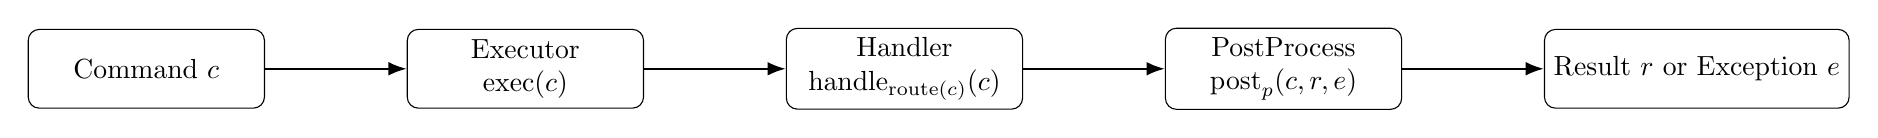
\begin{tikzpicture}[
  node distance=1.8cm and 1.8cm,
  every node/.style={draw, rectangle, rounded corners, align=center, minimum width=3cm, minimum height=1cm},
  arrow/.style={-Latex, thick}
]
\node (command) {Command $c$};
\node (executor) [right=of command] {Executor\\ $\mathrm{exec}(c)$};
\node (handler) [right=of executor] {Handler\\ $\mathrm{handle}_{\mathrm{route}(c)}(c)$};
\node (post) [right=of handler] {PostProcess\\ $\mathrm{post}_p(c, r, e)$};
\node (result) [right=of post] {Result $r$ or Exception $e$};

\draw[arrow] (command) -- (executor);
\draw[arrow] (executor) -- (handler);
\draw[arrow] (handler) -- (post);
\draw[arrow] (post) -- (result);

\end{tikzpicture}
\end{center}

\section{Best Practices}
Use Command Pattern consistently for all operations.

Keep middleware lightweight and composable.

Use Disruptor or equivalent event-driven infrastructure for high throughput.

Apply Strategy or Template patterns to standardize command execution.

Monitor performance, latency, and exception handling.

\section{Conclusion and Future Work}
Summarize contributions: pattern mapping, trade-offs, implementation guide.

\subsection{Future directions}
Distributed CQRS with multiple nodes

Event sourcing integration

AI-assisted command routing and pattern detection

\bibliographystyle{alpha}
\bibliography{sample}
\end{document}
